\documentclass[dvipdfmx]{article}
\usepackage{geometry}
\geometry{a4paper, top=1.0cm, left=2.5cm, right=2.5cm, bottom=1cm, includefoot}

\usepackage[dvipdfmx]{graphicx, xcolor}
\usepackage{here}
\usepackage{color}
\usepackage{xcolor}
\usepackage{amsmath, amssymb, bm}
\usepackage{amsthm}
\usepackage{cases}
\usepackage{cite}
\usepackage{enumitem}
\usepackage{mathtools}
\usepackage{multirow}
\usepackage{bbm}
\usepackage{ascmac}
\usepackage{arydshln}
\usepackage[table]{xcolor}
\usepackage{float}
\usepackage{fancybox}
\usepackage{caption}
\usepackage{mdframed}
\usepackage{hyperref}
\usepackage{algorithm,algorithmic}
\usepackage{wrapfig}
\usepackage{url}
\usepackage{indentfirst}
\usepackage{stmaryrd}
\usepackage{braket}
\usepackage{booktabs}
\usepackage{siunitx} % 数値列の整列に便利
\usepackage{mathcomp}
\usepackage{subfig}


\graphicspath{{fig/}}
%\usepackage{color}
\captionsetup{justification=centering}

\newtheorem{theorem}{定理}
\newtheorem{lemma}[theorem]{補題}
\renewcommand{\figurename}{図}
\renewcommand{\abstractname}{Abstract}
\newcommand{\la}{\lambda}
\newcommand{\li}{\lambda_i}
\newcommand{\argmax}{\mathop{\rm arg~max}\limits}
\newcommand{\argmin}{\mathop{\rm arg~min}\limits}

\newcommand{\ds}{\displaystyle}
\newcommand{\dd}{\mathrm{d}}
\newcommand{\E}{\mathrm{E}}
\newcommand{\one}{\mathbbm{1}}
\newcommand{\bb}{\mathbb{R}}

\DeclareGraphicsRule{.tif}{png}{.png}{`convert #1 `dirname #1`/`basename #1 .tif`.png}
% Vectors

\newcommand{\av}{\mathbf{a}}
\newcommand{\bv}{\mathbf{b}}
\newcommand{\cv}{\mathbf{c}}
\newcommand{\dv}{\mathbf{d}}
\newcommand{\ev}{\mathbf{e}}
\newcommand{\fv}{\mathbf{f}}
\newcommand{\gv}{\mathbf{g}}
\newcommand{\hv}{\mathbf{h}}
\newcommand{\iv}{\mathbf{i}}
\newcommand{\jv}{\mathbf{j}}
\newcommand{\kv}{\mathbf{k}}
\newcommand{\lv}{\mathbf{l}}
\newcommand{\mv}{\mathbf{m}}
\newcommand{\nv}{\mathbf{n}}
\newcommand{\ov}{\mathbf{o}}
\newcommand{\pv}{\mathbf{p}}
\newcommand{\qv}{\mathbf{q}}
\newcommand{\rv}{\mathbf{r}}
\newcommand{\sv}{\mathbf{s}}
\newcommand{\tv}{\mathbf{t}}
\newcommand{\uv}{\mathbf{u}}
\newcommand{\wv}{\mathbf{w}}
\newcommand{\vv}{\mathbf{v}}
\newcommand{\xv}{\mathbf{x}}
\newcommand{\yv}{\mathbf{y}}
\newcommand{\zv}{\mathbf{z}}
\newcommand{\zerov}{\mathbf{0}}
\newcommand{\onev}{\mathbf{1}}

% Matrices

\newcommand{\Am}{\mathbf{A}}
\newcommand{\Bm}{\mathbf{B}}
\newcommand{\Cm}{\mathbf{C}}
\newcommand{\Dm}{\mathbf{D}}
\newcommand{\Em}{\mathbf{E}}
\newcommand{\Fm}{\mathbf{F}}
\newcommand{\Gm}{\mathbf{G}}
\newcommand{\Hm}{\mathbf{H}}
\newcommand{\Id}{\mathbf{I}}
\newcommand{\Jm}{\mathbf{J}}
\newcommand{\Km}{\mathbf{K}}
\newcommand{\Lm}{\mathbf{L}}
\newcommand{\Mm}{\mathbf{M}}
\newcommand{\Nm}{\mathbf{N}}
\newcommand{\Om}{\mathbf{O}}
\newcommand{\Pm}{\mathbf{P}}
\newcommand{\Qm}{\mathbf{Q}}
\newcommand{\Rm}{\mathbf{R}}
\newcommand{\Sm}{\mathbf{S}}
\newcommand{\Tm}{\mathbf{T}}
\newcommand{\Um}{\mathbf{U}}
\newcommand{\Wm}{\mathbf{W}}
\newcommand{\Vm}{\mathbf{V}}
\newcommand{\Xm}{\mathbf{X}}
\newcommand{\Ym}{\mathbf{Y}}
\newcommand{\Zm}{\mathbf{Z}}
\newcommand{\Lam}{\mathbf{\Lambda}}

% Calligraphic
\newcommand{\Ac}{\mathcal{A}}
\newcommand{\Bc}{\mathcal{B}}
\newcommand{\Cc}{\mathcal{C}}
\newcommand{\Dc}{\mathcal{D}}
\newcommand{\Ec}{\mathcal{E}}
\newcommand{\Fc}{\mathcal{F}}
\newcommand{\Gc}{\mathcal{G}}
\newcommand{\Hc}{\mathcal{H}}
\newcommand{\Ic}{\mathcal{I}}
\newcommand{\Jc}{\mathcal{J}}
\newcommand{\Kc}{\mathcal{K}}
\newcommand{\Lc}{\mathcal{L}}
\newcommand{\Mc}{\mathcal{M}}
\newcommand{\Nc}{\mathcal{N}}
\newcommand{\Oc}{\mathcal{O}}
\newcommand{\Pc}{\mathcal{P}}
\newcommand{\Qc}{\mathcal{Q}}
\newcommand{\Rc}{\mathcal{R}}
\newcommand{\Sc}{\mathcal{S}}
\newcommand{\Tc}{\mathcal{T}}
\newcommand{\Uc}{\mathcal{U}}
\newcommand{\Wc}{\mathcal{W}}
\newcommand{\Vc}{\mathcal{V}}
\newcommand{\Xc}{\mathcal{X}}
\newcommand{\Yc}{\mathcal{Y}}
\newcommand{\Zc}{\mathcal{Z}}
\newcommand{\Ecb}{\mathbf{\mathcal{E}}}
\newcommand{\Ocb}{\mathbf{\mathcal{O}}}
\newcommand{\Lcb}{{\bm \mathcal{L}}}

% Bold greek letters

\newcommand{\alphav}{\hbox{\boldmath$\alpha$}}
\newcommand{\betav}{\hbox{\boldmath$\beta$}}
\newcommand{\gammav}{\hbox{\boldmath$\gamma$}}
\newcommand{\deltav}{\hbox{\boldmath$\delta$}}
\newcommand{\etav}{\hbox{\boldmath$\eta$}}
\newcommand{\lambdav}{\hbox{\boldmath$\lambda$}}
\newcommand{\epsilonv}{\hbox{\boldmath$\epsilon$}}
\newcommand{\nuv}{\hbox{\boldmath$\nu$}}
\newcommand{\muv}{\hbox{\boldmath$\mu$}}
\newcommand{\zetav}{\hbox{\boldmath$\zeta$}}
\newcommand{\phiv}{\hbox{\boldmath$\phi$}}
\newcommand{\psiv}{\hbox{\boldmath$\psi$}}
\newcommand{\thetav}{\hbox{\boldmath$\theta$}}
\newcommand{\tauv}{\hbox{\boldmath$\tau$}}
\newcommand{\omegav}{\hbox{\boldmath$\omega$}}
\newcommand{\xiv}{\hbox{\boldmath$\xi$}}
\newcommand{\sigmav}{\hbox{\boldmath$\sigma$}}
\newcommand{\piv}{\hbox{\boldmath$\pi$}}
\newcommand{\rhov}{\hbox{\boldmath$\rho$}}

\newcommand{\Gammam}{\hbox{\boldmath$\Gamma$}}
\newcommand{\Lambdam}{\hbox{\boldmath$\Lambda$}}
\newcommand{\Deltam}{\hbox{\boldmath$\Delta$}}
\newcommand{\Sigmam}{\hbox{\boldmath$\Sigma$}}
\newcommand{\Phim}{\hbox{\boldmath$\Phi$}}
\newcommand{\Pim}{\hbox{\boldmath$\Pi$}}
\newcommand{\Psim}{\hbox{\boldmath$\Psi$}}
\newcommand{\Thetam}{\hbox{\boldmath$\Theta$}}
\newcommand{\Omegam}{\hbox{\boldmath$\Omega$}}
\newcommand{\Xim}{\hbox{\boldmath$\Xi$}}

% mixed symbols

% \newcommand{\sinc}{{\hbox{sinc}}}
% \newcommand{\diag}{{\hbox{diag}}}
% \renewcommand{\det}{{\hbox{det}}}
% \newcommand{\trace}{{\hbox{tr}}}
% \newcommand{\sign}{{\hbox{sign}}}
% \renewcommand{\arg}{{\hbox{arg}}}
% \newcommand{\var}{{\hbox{var}}}
% \newcommand{\cov}{{\hbox{cov}}}
% \newcommand{\SINR}{{\sf SINR}}
% \newcommand{\SNR}{{\sf SNR}}
% \newcommand{\Ei}{{\rm E}_{\rm i}}
% \renewcommand{\Re}{{\rm Re}}
% \renewcommand{\Im}{{\rm Im}}
% \newcommand{\eqdef}{\stackrel{\Delta}{=}}
% \newcommand{\defines}{{\,\,\stackrel{\scriptscriptstyle \bigtriangleup}{=}\,\,}}
% \newcommand{\<}{\left\langle}
% \renewcommand{\>}{\right\rangle}
% \newcommand{\herm}{{\sf H}}
% \newcommand{\transp}{{\sf T}}
% \renewcommand{\vec}{{\rm vec}}


% New theorem environments
% \newtheorem{theorem}{Theorem}
% \newtheorem{conjecture}{Conjecture}
% \newtheorem{proposition}{Proposition}
% \newtheorem{lemma}{Lemma}
% \newtheorem{definition}{Definition}
% \newtheorem{corollary}{Corollary}
% \newtheorem{objective}{Objective}
% \newtheorem{observation}{Observation}

% \newcommand{\E}[1]{\mathbb{E}\left\{{#1}\right\}}
% \newcommand{\Var}[1]{\text{Var}\left\{{#1}\right\}}
% \newcommand{\Tr}[1]{\text{Tr}\left({#1}\right)}
% \newcommand{\defeq}{\stackrel{\triangle}{=}}


% \DeclareMathOperator*{\argmin}{arg\,min}
% \DeclareMathOperator*{\argmax}{arg\,max}




\title{Progress Report}
\author{林 奏汰}
\date{2026/4/10}

\begin{document}

\maketitle


% \begin{abstract}
% 人は，環境に潜む規則性を意識せずとも自然に習得する能力を有しており，これは暗黙的学習と呼ばれる．
% 前回の進捗報告では，反応時間の変動係数を注意状態の個人差指標として用い，学習指標との関係を検討した．
% その結果，注意状態が不安定な参加者ほど暗黙的学習の進行が促進されることが示唆された．
% 本報告では，そのメカニズムとして試行レベルの注意変動が媒介している可能性について検討する．
% 具体的には，反応時間の時系列から試行ごとの注意状態をラベル付けし，Q学習モデルを用いて注意状態ごとに学習の進行度合いを定量化することを試みた．
% その結果，注意が散漫状態における学習率は集中状態よりも高い傾向が認められたが，その差分と反応時間の変動係数との間に有意な関係は確認されなかった．
% \end{abstract}

\section{\textcolor{red}{Introduction}}
Humans possess the ability to naturally acquire regularities embedded in their environment without conscious awareness.
This phenomenon, known as implicit learning, plays an important role in various domains, including language acquisition and motor skill learning~\cite{cleeremans1998implicit,frensch2003implicit,maresch2021measures,costea2023implicit}.

Substantial individual differences have been observed in the process of acquiring implicit regularities~\cite{kalra2019evidence}.
In our previous progress report, we used the coefficient of variation (CV) of reaction time as an individual-difference index of attentional state and examined its relationship with a learning index.
The results showed that participants with a larger RT-CV exhibited a significantly greater increase in the proportion of choices toward the high-reward dot cluster as the task progressed.
This result suggests that fluctuations in attentional state influence the progression of implicit learning.
In this report, we examine the possibility that trial-level attentional fluctuations mediate this mechanism.

A study on mind wandering has proposed a method for labeling the attentional state on each trial based on the time series of reaction times~\cite{decker2023pay}.
In this method, a trial is defined as being in an Out-Of-the-Zone (OOZ) state—i.e., a state of attentional lapse—if the moving average of reaction times over the preceding trials is shorter than the individual's mean and the local variability is larger than a threshold; the attentional state is thereby determined on a trial-by-trial basis.
To test whether trial-level attentional fluctuations mediate learning, it is necessary to compare the degree of learning progression between attentional states.
We therefore estimated, using a Q-learning model, the learning rate for each attentional state and examined whether the degree of learning progression differed between the OOZ and non-OOZ states.
We further examined whether the difference between these learning rates was related to the coefficient of variation of reaction time.

The results showed a tendency for the learning rate in the OOZ state to be higher than that in the non-OOZ state, although this difference was not significantly related to the coefficient of variation of reaction time.
This result suggests that trial-level attentional fluctuations and individual-level attentional traits may contribute independently to implicit learning.


\section{Experiment}
\begin{figure}[t]
    \centering
    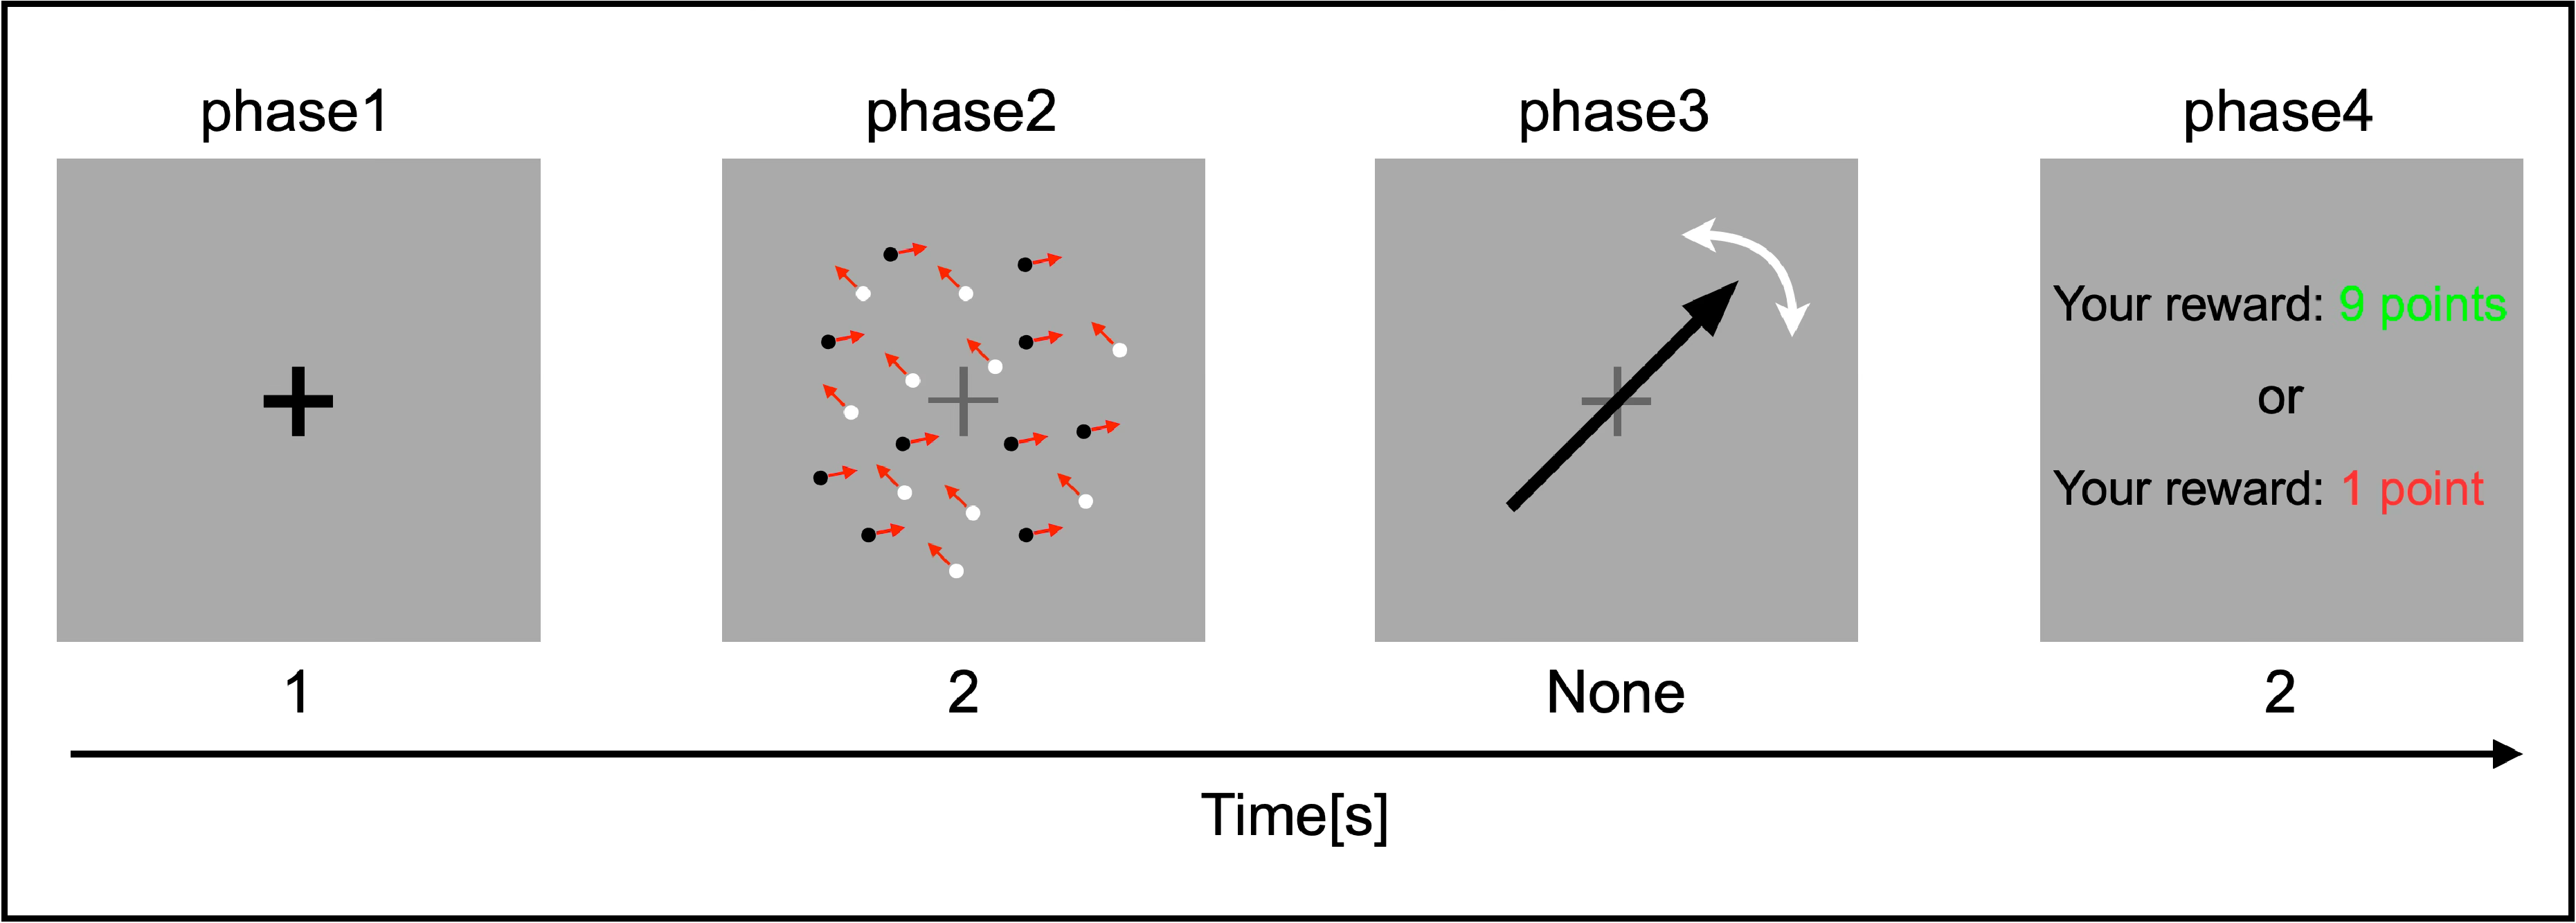
\includegraphics[width=1.0\textwidth]{../assets/dual-rdk-procedure-modified.pdf}
    \caption{Experiment procedure.}
    \label{fig:experiment_procedure}
\end{figure}

\subsection{Environment}
The experiment was created using JsPsych v2.0.0.

\subsection{Participants}
A total of 80 participants were recruited using the online experiment tool Prolific~\cite{palan2018prolific}.

\subsection{Experimental Procedure}
The experiment consisted of a 16-trial practice session and a 72-trial main session.
The procedure for each trial is illustrated in Figure~\ref{fig:experiment_procedure}.
Each trial consisted of the presentation of a fixation point, the simultaneous presentation of two RDK stimuli with different colors (white and black), a direction response phase, and a reward phase.

Participants were presented with two types of RDK stimuli that moved in different directions—one white and one black—and were instructed to report the direction of the dot cluster with more dots.
In other words, in this task, the stimulus with more dots was the target stimulus, and the stimulus with fewer dots was the distractor stimulus.
Each trial consisted of four phases: fixation point presentation (1 second), stimulus presentation (2 seconds), response, and reward presentation (2 seconds).
The fixation point was designed to guide participants' gaze to the center of the screen and reduce variability in eye movements before stimulus presentation.
During the stimulus presentation phase, the white and black RDK stimuli were presented simultaneously,
and during the response phase, participants were instructed to rotate a bar using the left and right arrow keys on the keyboard,
aligning its orientation with the direction of movement of the dot cluster.
The initial position of the bar was randomly determined, and response time was unlimited.
In the reward phase, a reward was presented based on the angular error relative to the target stimulus
(the method for determining the reward is described in Section~\ref{sec:reward_structure}).
Participants were informed in advance that they would receive compensation after the experiment based on the total reward they had obtained.
The experiment took approximately 15 minutes to complete.

\subsubsection{Practice Session}
The practice session consisted of 16 trials and was intended to familiarize participants with operating the bar.
The number of dots and the direction of motion were determined randomly, and two RDK stimuli of different luminance were presented simultaneously.
Thus, in the practice session, the difference in dot number between the two dot clusters was clearly noticeable.

\subsubsection{Main Session}
The main session consisted of 72 trials, with the first 48 trials constituting the learning stage and the remaining 24 trials constituting the awareness stage.
On each trial of the main session, two RDK stimuli of different colors with an equal number of dots were presented simultaneously.
That is, because the two RDK stimuli contained the same number of dots, there was no distinction between a target stimulus and a distractor stimulus based on dot number.
However, the direction of motion differed between the two colored dot clusters, and the reward was set to vary depending on this direction of motion.
Accordingly, in the main session, participants were instructed to report the direction of motion of the dot cluster that appeared to contain more dots, even though, in reality, the reward depended not on dot number but on direction of motion.
The reward structure of the main session is described in the next section.



\subsection{Reward Structure}\label{sec:reward_structure}
The reward structure in the main session was not explicitly communicated to participants,
and participants needed to learn the implicitly set reward structure to obtain higher rewards.

\begin{figure}[t]
    \centering
    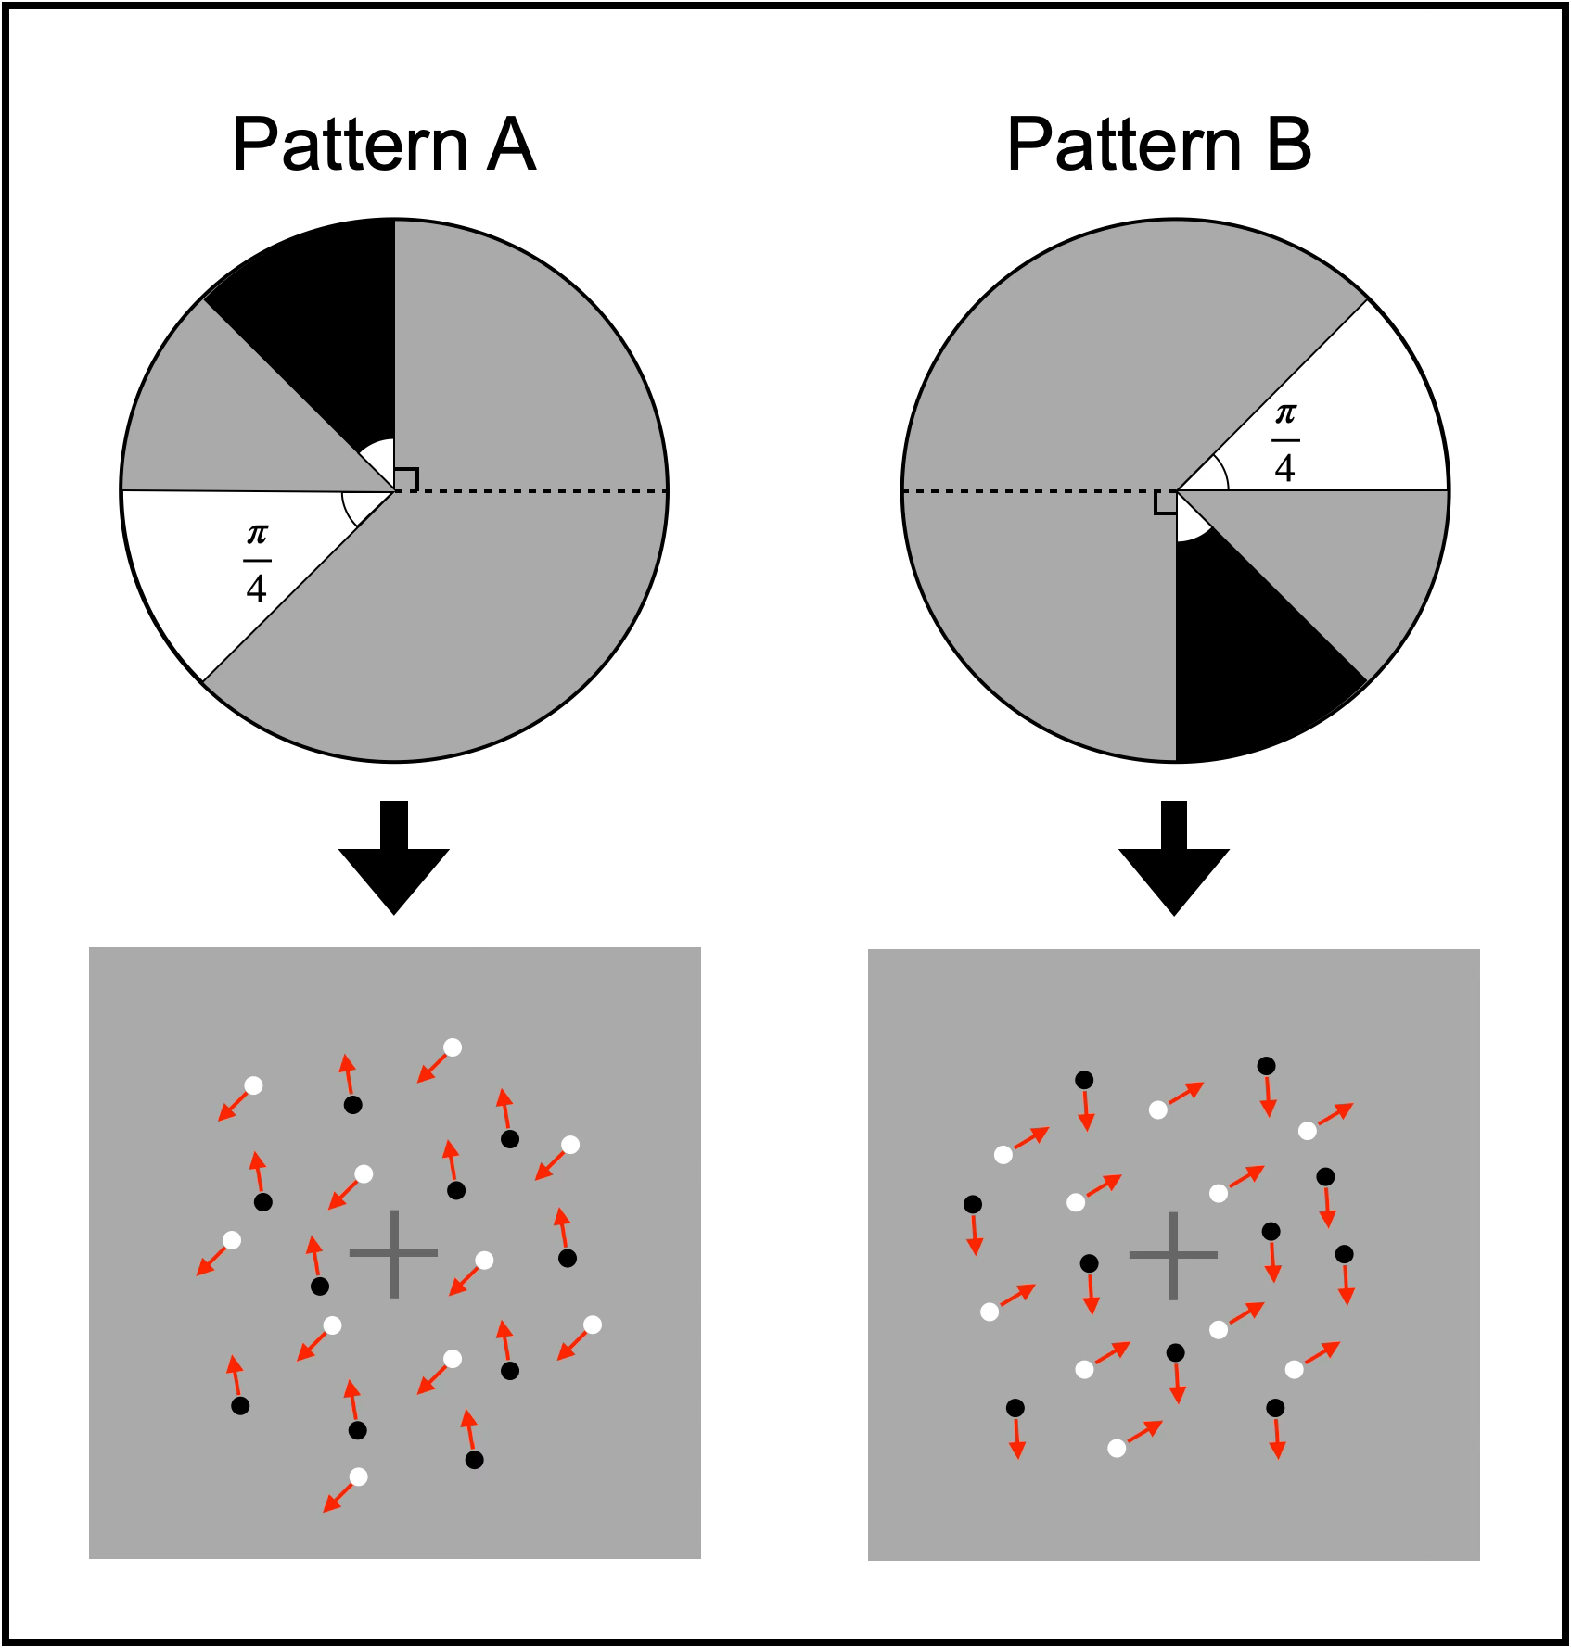
\includegraphics[width=0.5\linewidth]{../assets/learning-stimuli-modified.pdf}
    \caption{Main session stimulus patterns.
    (Top) The range of motion directions for white and black dot clusters.
    (Bottom) Specific examples of stimuli (red arrows indicate the motion direction of the dot clusters).
    % For the right-side pairs, the white dot cluster is the target, and the black dot cluster is the distractor\\
    % For the left-side pairs, the black dot cluster is the target, and the white dot cluster is the distractor
    }
    \label{fig:stimuli}
\end{figure}
The stimuli in each trial of the main session were composed of high-reward and low-reward stimuli.
Each of these stimuli had a pattern with a certain regularity, and there were two types of patterns.
Figure~\ref{fig:stimuli} shows the patterns of the two types of stimuli in the main session, the range of motion directions for the dot clusters, and specific examples of the stimuli.
In Pattern A, the high-reward stimulus is the black dot cluster, and the low-reward stimulus is the white dot cluster.
Conversely, in Pattern B, the high-reward stimulus is the white dot cluster, and the low-reward stimulus is the black dot cluster.
In each trial, one of these two types of stimuli patterns was randomly selected and presented.
The range of motion directions for each stimulus was $\pi/4$, and the angular distance between the high-reward and low-reward stimuli was $\pi/4$.

The reward for each trial was adjusted so that if the response angle matched the target direction angle, 10 points were awarded, and if it deviated by $\pi/4$ or more, 0 points were awarded.
To achieve this, a constraint was imposed on each trial such that the angle between the motion directions of the two dot clusters was always at least $\pi/2$.
This ensured that even if participants correctly reported the target,
their responses would not be confused with those of the distractor.

\subsection{Stage Design}
This section describes the design of the learning stage and awareness stage in the main session.

The learning stage aimed to verify whether participants could implicitly learn the reward structure.
Participants were not explicitly informed about the existence of the reward structure,
and their ability to learn it was assessed by measuring the proportion of high-reward dot clusters selected over repeated trials.
Participants were not explicitly informed about the existence of the reward structure,
and their ability to learn it was assessed by measuring the proportion of high-reward dot clusters selected over repeated trials.

The awareness stage aimed to verify whether the learning observed in the learning stage was based on conscious knowledge.
Therefore, the reward structure in the awareness stage was designed as a rotation of the structure from the learning stage by $\pi$ radians,
resulting in a structure where the high-reward and low-reward dot clusters were swapped.
If the knowledge acquired during the learning stage was conscious, participants would be expected to notice the reversal of the reward structure and change their choice behavior accordingly.
On the other hand, if the learning was unconscious, the previous choice tendency would be expected to persist even after the reversal of the reward structure.

In the analyses that follow, we refer to the high-reward stimulus in the main session as the target stimulus for convenience,
and define the proportion of trials on which the high-reward stimulus was chosen as the target choice rate.


\section{\textcolor{red}{Computational Framework}}
In this study, following the method of a previous study~\cite{decker2023pay}, we labeled the attentional state on each trial based on the time series of reaction times,
and further attempted to quantify the degree of learning progression for each attentional state using a Q-learning model.

\subsection{Labeling of Attentional States}\label{sec:attention_labeling}
In the method of decker et al.~\cite{decker2023pay}, a trial is regarded as being in a state of distraction (Out Of the Zone: OOZ) if the moving average of reaction times over the preceding trials is short and deviates from the participant's typical pattern, and the attentional state is estimated on a trial-by-trial basis.
Specifically, a trial is defined as OOZ if the moving average of reaction times over the preceding $N$ trials is shorter than the participant's overall mean (i.e., the level is low),
and the moving average of reaction time deviations over the preceding $N$ trials is larger than a threshold computed across participants (i.e., the variability is high).
Note that trials with $t < N$ were excluded from the analysis, since fewer than $N$ trials would be available for the moving average.
The original study used $N=3$.



Definition of Index A (level):

$$M_t = \frac{1}{N}\sum_{k=1}^{N} \text{RT}_{t-k}$$

Definition of Index B (variability):

$$D_t = \frac{1}{N}\sum_{k=1}^{N} \left|\text{RT}_{t-k} - \bar{\mu}_i\right|$$

Here, $\bar{\mu}_i$ denotes the mean $\text{RT}$ of participant $i$ across all trials.

Definition of the thresholds:

$$\bar{M}^{(i)} = \frac{1}{T}\sum_{t=1}^T M_t^{(i)}, \quad D^* = \frac{1}{P}\sum_{i=1}^P \text{median}_t\left(D_t^{(i)}\right)$$

Here, $T$ denotes the number of trials and $P$ denotes the number of participants.

Definition of the OOZ label:

$$\text{OOZ}_{t}^{(i)} = \mathbf{1}\big[ M_t < \bar{M}^{(i)}\big] \cdot \mathbf{1}\big[D_t > D^*\big]$$

Here, $\mathbf{1}[\cdot]$ denotes the indicator function, which returns 1 if the condition inside the brackets is true and 0 otherwise.
Thus, $\text{OOZ}_{t}^{(i)} = 1$ holds only for trials on which the level of reaction time is lower than the participant's own mean ($M_t < \bar{M}^{(i)}$) and the variability of reaction time is larger than the threshold computed across participants ($D_t > D^*$).

\subsection{Application of the Q-Learning Model}
The Q-learning model is a reinforcement learning framework in which an agent sequentially learns an action-selection policy that maximizes the reward obtained from the environment.
In this study, we applied the Q-learning model to participants' color choices and reward histories to estimate each participant's learning rate.
In what follows, we first formulate the basic model, then introduce the color bias term and compare the resulting models, and finally describe the extension to the attentional-state-dependent learning rate model.


\subsubsection{Basic Model}

\paragraph{Definition of States, Actions, and Q-Values}
The state $s_t \in \{0, 1\}$ denotes the reward-structure pattern on trial $t$
($s_t = 0$: white is high-reward, $s_t = 1$: black is high-reward).
The action $a_t \in \{0, 1\}$ denotes the color chosen by the participant
($a_t = 0$: white, $a_t = 1$: black).
We maintain a Q-value table $Q_t(s, a)$ for each state-action pair, with all initial values set to $0.5$:
\begin{equation}
    Q_1(s, a) = 0.5 \quad \forall\, s, a
\end{equation}

\paragraph{Choice Probability}
The action-selection probability on trial $t$ is determined by a softmax function based on the difference in Q-values:
\begin{equation}
    \Delta Q_t = \beta \left( Q_t(s_t, 1) - Q_t(s_t, 0) \right)
\end{equation}
\begin{equation}
    P(\text{target} \mid s_t, Q_t) =
    \begin{cases}
        \sigma(-\Delta Q_t) & (s_t = 0) \\
        \sigma(+\Delta Q_t) & (s_t = 1)
    \end{cases}
\end{equation}
Here, $\sigma(x) = 1/(1 + e^{-x})$ is the sigmoid function, and $\beta > 0$ is the inverse temperature parameter.

\paragraph{Q-Value Update}
After receiving reward $r_t$, the Q-value of the chosen state-action pair is updated according to the following rule:
\begin{equation}
    Q_{t+1}(s_t, a_t) = Q_t(s_t, a_t) + \alpha \left( r_t - Q_t(s_t, a_t) \right)
\end{equation}
Here, $\alpha \in (0, 1)$ is the learning rate; a larger value indicates that more recent rewards are weighted more heavily.
The Q-values of all other state-action pairs remain unchanged.

\subsubsection{Introduction of the Color Bias Term}

In the basic model, only the target stimulus yields a positive reward, so the Q-value of the distractor converges to $0$ as trials progress.
Owing to this structure, the basic model cannot produce a target choice probability below $0.5$.
In practice, however, some participants exhibit a persistent preference for a particular color (white or black).
To represent such a state-independent, stationary color bias, we introduced an additive term $c_\mathrm{black}$ to the log-odds:
\begin{equation}
    \Delta Q_t = \beta \left( Q_t(s_t, 1) - Q_t(s_t, 0) \right) + c_\mathrm{black}
\end{equation}
$c_\mathrm{black} > 0$ indicates a preference for black, and $c_\mathrm{black} < 0$ indicates a preference for white.
Because this term is added to the log-odds independently of $\beta$, it can be interpreted as a stationary bias that is independent of decision confidence.

\paragraph{Comparison with the Basic Model}
Table~\ref{tab:model_comparison} shows the results of comparing the goodness of fit between the basic model ($\alpha, \beta$; $k=2$) and the color bias model ($\alpha, \beta, c_\mathrm{black}$; $k=3$) ($n=54$).

\begin{table}[h]
    \centering
    \caption{Comparison of goodness of fit between the basic model and the color bias model (mean values, $n=54$)}
    \label{tab:model_comparison}
    \begin{tabular}{lS[table-format=-2.2]S[table-format=2.2]S[table-format=2.1]}
        \toprule
        Model & {Log-likelihood} & {AIC} & {Choice accuracy (\%)} \\
        \midrule
        Basic model ($k=2$)      & -26.37 & 56.75 & 61.6 \\
        Color bias model ($k=3$) & -23.39 & 52.77 & 73.2 \\
        \midrule
        Improvement & {$+2.99$} & {$-3.98$} & {$+11.6$ pp} \\
        \bottomrule
    \end{tabular}
\end{table}

The AIC improved by $-3.98$ for the color bias model, indicating that this model was superior in terms of both the information criterion and predictive accuracy.
This suggests that introducing the color bias term allows the model to appropriately describe the behavior of participants whose target choice rate falls below chance level.


\subsubsection{Attentional-State-Dependent Model}

We further extended the color bias model by constructing a model in which the learning rate switches according to the attentional state labeled in Section~\ref{sec:attention_labeling}.
Based on the OOZ label $z_t \in \{0, 1\}$, the Q-value update rule is defined as follows:
\begin{equation}
    Q_{t+1}(s_t, a_t) = Q_t(s_t, a_t) + \alpha_{z_t} \left( r_t - Q_t(s_t, a_t) \right)
\end{equation}
Here, $\alpha_0 \in (0,1)$ is the learning rate in the non-OOZ state (focused state), and $\alpha_1 \in (0,1)$ is the learning rate in the OOZ state (distracted state).
The model thus has four parameters: $(\alpha_0, \alpha_1, \beta, c_\mathrm{black})$.

\paragraph{MAP Estimation}
We placed the following priors on each parameter and performed MAP estimation by maximizing the log posterior probability:
\begin{align}
    \alpha_0, \alpha_1 &\sim \mathrm{Beta}(2, 2) \\
    \beta               &\sim \mathrm{Gamma}(2, 3) \\
    c_\mathrm{black}    &\sim \mathcal{N}(0, 2)
\end{align}
Optimization was performed using the L-BFGS-B method, with a grid search over multiple initial values to avoid local optima.

\section{\textcolor{red}{Analysis}}
\begin{table}[h]
    \centering
    \caption{Comparison of goodness of fit between the color bias model and the attentional-state-dependent model (mean values, $n=54$)}
    \label{tab:model_comparison_ooz}
    \begin{tabular}{lS[table-format=-2.2]S[table-format=2.2]S[table-format=2.1]}
        \toprule
        Model & {Log-likelihood} & {AIC} & {Choice accuracy (\%)} \\
        \midrule
        Color bias model ($k=3$)               & -23.39 & 52.77 & 73.2 \\
        Attentional-state-dependent model ($k=4$) & -23.25 & 54.49 & 73.1 \\
        \midrule
        Improvement & {$+0.14$} & {$+1.72$} & {$-0.1$ pp} \\
        \bottomrule
    \end{tabular}
\end{table}
First, Table~\ref{tab:model_comparison_ooz} shows the results of comparing the goodness of fit between the attentional-state-dependent model ($\alpha_0, \alpha_1, \beta, c_\mathrm{black}$; $k=4$) and the color bias model ($\alpha, \beta, c_\mathrm{black}$; $k=3$) ($n=54$).
Although the log-likelihood improved slightly ($+0.14$), this improvement fell short of the AIC penalty associated with the additional parameter ($+2$), and the AIC worsened by $+1.72$. The choice accuracy showed almost no change ($-0.1$ pp).
These results suggest that extending the model to incorporate attentional-state dependence does not improve the overall goodness of fit.

Next, to examine whether the learning rate differed between the OOZ and non-OOZ states, we tested, using a one-sample $t$-test, the null hypothesis that the across-participant mean of the estimated learning-rate difference $\Delta\alpha = \alpha_1 - \alpha_0$ was equal to 0.
The result did not reach statistical significance, but a trend was observed in which $\alpha_1$ was higher than $\alpha_0$ ($t(53) = 1.82, p = 0.07$).
That is, a trend was observed in which the learning rate in the OOZ state was higher than that in the non-OOZ state.

\begin{figure}[t]
    \centering
    
\includegraphics[width=0.8\textwidth]{../../outputs/figures/rt_cv_vs_alpha_diff.pdf}
    \caption{Relationship between the index of learning progression and the coefficient of variation of reaction time.}
    \label{fig:rt_cv_vs_alpha_diff}
\end{figure}
Finally, using $\Delta\alpha$ as an index of learning progression, we examined its relationship with the coefficient of variation of reaction time (${\text{CV}}_{\text{RT}}$).
The results showed no significant relationship between the learning-rate difference and the variability of reaction time (Figure~\ref{fig:rt_cv_vs_alpha_diff}).


\section{\textcolor{red}{Discussion}}
In this report, we examined the possibility that trial-level attentional fluctuations mediate implicit learning.
The results showed a trend toward a higher learning rate in the OOZ state than in the non-OOZ state ($p = 0.07$), but no significant relationship was found between the learning-rate difference and the coefficient of variation of reaction time.

To interpret the trend toward a higher learning rate in the OOZ state, it is necessary to consider the two conditions used to define OOZ.
In the OOZ criterion, trials with a low level of reaction time and large local variability are extracted as the distracted state.
According to the definition used in the previous study~\cite{decker2023pay}, the condition of a low level corresponds to selectively capturing trials in which an impulsive response occurred without deliberation.
On such trials, weakened selective processing of the stimuli may loosen the focusing of attention on a single dot cluster, allowing the contingency between both stimuli's information and the reward feedback to be encoded more broadly.
In other words, although perceptual accuracy may be sacrificed, the broadened input regarding the reward structure could act to increase the learning rate.
This interpretation, in which a relaxation of attentional focus promotes implicit learning, is consistent with recent research on mind wandering.
Simor et al.~\cite{simor2025mind} have suggested that mind wandering broadens the scope of attention, thereby promoting the exploration of probabilistic contingencies in the environment when the task's rules or goals are not explicit.
However, the task used in this study involves responses requiring perceptual judgment, and unlike the simple response tasks used in previous studies, the directionality of reaction time in the distracted state is not self-evident.
Therefore, whether faster responses correspond to the distracted state in this task requires separate verification.

On the other hand, the absence of a relationship between the learning-rate difference and the coefficient of variation of reaction time suggests that trial-level attentional state and individual-level attentional traits may reflect different components.
The OOZ criterion is an index that selectively captures only local fluctuations on the faster side of reaction time variability, whereas the coefficient of variation of reaction time reflects overall instability, including slower-side variability and gradual transitions between states.
Therefore, the learning index derived via the OOZ criterion does not necessarily capture the learning-related component reflected in the coefficient of variation of reaction time.

Taken together, these results suggest that trial-level attentional fluctuations (OOZ) and individual-level attentional traits (coefficient of variation of reaction time) may contribute independently to implicit learning.


\clearpage
\bibliographystyle{unsrt}
\bibliography{myrefs}

\end{document}